\chapter{Feature selection}

In order to create an effective predictive model one must first select a set of features used to produce each classification. Both a science and an art, this process involves intuition, theory and a hefty amount of trial-and-error. Although a seemingly daunting task, for a model to be effective the feature selection procedure is key, and a carefully considered selection often generates significantly better results than one put together without much thought. 

Ideally, one seeks a small set of variables which accurately captures the information content in some larger set of data. After reducing the number of features into a more manageable format it is then possible to obtain good results with significantly less computational load than if no feature selection had been considered. 
%Furthermore, the feature selection process allows us to pinpoint what data characteristics we wish to monitor, and subsequently which data characteristics we can disregard. 

\section{An impossible modeling problem}

Fundamentally, the radar used transmits pulses with some envelope $A(t)$ of some frequency $\Omega$ into its surroundings.

\begin{equation}
	x(t) = A(t)\sin(\Omega t + \varphi)
\end{equation}

After scattering, a signal $s(t)$ reaches the receiving antenna. This signal is comprised of radiation diffuesly scattered from the target scene. It contains both specular (i.e. mirror-like) and non-specular reflective components. Its content will be a function dependant both on the surrounding surface topography, as well as the dielectric properties of the surface at hand \citep{grossman_popovic_chamberlin_gordon_novotny_2017}. Furthermore, the surfaces at hand have a, to some degree, random structure with varying characteristics. The great difficulty with modeling $s(t)$ is clear - the universe of all possible "realistic" surfaces, both natural and man-made, is almost impossibly large. Without making significant assumptions with regards to surface roughness or dielectric properties, there is no general model of $s(t)$ we can make use of. Instead, we have to come up with a set of \emph{reasonable} features that \emph{should} capture the signal structure. These features will no be based on any specific signal model, but instad rely on the returning signals having stable structure over brief periods of time. Hence our task is to find \emph{defining characteristics} from a given surface using the sequence of one dimensional data obtained from a radar sensor. 


As the radar samples rather quickly at around 200 Hz we can allow ourselves to use a sequence of sweeps to generate one prediction. This allows for feature-processing over a number of sweeps, rather than on a sweep-by-sweep basis. Besides improving the signal-to-noise ratio \citep{w_doerry_2016} we may also investigate time correlations when using multiple radar sweeps. If $T$ sweeps are used per classification, the rate of classifications $F_c$ produced relates to the sampling rate $F_s$ through

\begin{equation}
	\label{eq:classification_rate}
	F_c = \frac{F_s}{T}
\end{equation} 
The parameter $T$ becomes a tradeoff between accuracy and classification rate. The more samples $T$ used per classification the higher the classification accuracy is, but with the cost of a lower classification frequency. Conversely we may be able to generate feature estimates more rapidly by setting $T$ to a lower value, but will in the process end up with worse feature estimates. 

\section{Features}

The reflectivity of a material, described by its dielectric constant, shows up in the obtained IQ-demodulated sweeps in the amplitude of the returning signals. Therefore it might seem like a good idea to simply measure the energy content of a sweep and use it as a feature. However, due to inconsistencies inbetween individual sensors sweep normalization is performed as a pre-processing step rendering such calculations unusable. We are thus left with investigating the topography of the scene. 

In this section four different features are discussed aimed at capturing the geometric characteristics of a target surface. A radar datapoint captured at time $t$ and range $n$ is denoted as $x(n,t)$. Since we are using $T$ samples per classification, each new set of features $\mathbf{f}_m$ are estimated from time $t_m=Tm$ to $Tm+T-1$ 

\subsubsection{Expected signal}

First of all we may characterize a sweep by its envelope form - that is, the shape of the absolute values of the radar sweeps. If we can assume that the samples are taken from some unknown stochastic process $X_{n,t}$ with constant mean over $T$ samples we may for range $n$ and feature index $m$ form the estimate using $T$ consecutive sweeps to form the averaging estimate $s_n(m)$ through


\begin{equation}
	s_n(m) = \E\{X_{n,t_m}\}\frac{1}{T}\sum_{t=0}^{T-1}|x(n, t_m + t)|.
\end{equation}

These estimates form the expected signal feature vector $\mathbf{f}_{s,m}$ as 

\begin{equation}
	\mathbf{f}_{s,m} = 
	\begin{bmatrix}
		s_0(m) & s_1(m) & ... & s_{K-1}(m)
	\end{bmatrix}.
\end{equation}


In figure \ref{fig:sweep_average} we see what such an averaging process yields. Individual variances are suppressed to form a stable estimate of the sweep shape. 

\begin{figure}[h]
	\centering
	\includegraphics[scale=0.7]{figs_temp/features/sweep_average}
	\caption{By averaging a number of consecutive sweeps, we reduce noise and make samples more similar. The dashed line shows the average of the solid lines. }
	\label{fig:sweep_average}
\end{figure}


\subsubsection{Fourier Transform}
While traversing a static surface at a constant speed, one could think of it as the details on the surface, such as small rocks or grass, are moving closer to the radar sensor. This affects the transmitted radar waves according to the Doppler effect, and the radar detects \textit{Doppler frequencies}, corresponding to the frequency shifts. Depending on the surface's characteristics, the doppler frequencies may vary. 

One way to obtain the the frequency contents is by means of the discrete Fourier transform (DFT). In figure \ref{fig:fft}, typical DFTs are shown for all materials. The figure is intended to show differences in the DFTs. Hence, to make the difference more clear, the squre root of the DFT has been plotted. For grass (the top two plots), it can be seen that the frequency content is contained mainly at the zero frequency. The other materials contain slightly higher frequency content as well. Gravel, in particular, differs a lot from the other materials with a wide variety of frequency components.

As for the feature vector, a datasquare consisting of $T$ sweeps is selected. Viewing this as a matrix with elements $x(n,t)$, we can compute a $k$-step Fourier transform for each range, $n$, and sample index $m$, as
\begin{equation}
	\{\mathbb{X}^{(k)}_{n,m}\}_{k=0}^{T-1} =  \sum_{l=0}^{T-1}x(n,t_m+l)\exp\Big[-2\pi i\frac{kl}{T}\Big].
\end{equation}
After this, the absolute value of the Fourier transform is computed and the transformations of all ranges in the datasquare are concatenated into a one-dimensional feature vector of the form
\begin{equation}
	\textbf{f}_{f,m}=\begin{bmatrix} \{|\mathbb{X}_{0,m}^{(k)}|\}_{k=0}^{T-1} & \{|\mathbb{X}_{1,m}^{(k)}|\}_{k=0}^{T-1} & \hdots & \{|\mathbb{X}_{R,m}^{(k)}|\}_{k=0}^{T-1} \end{bmatrix},
\end{equation}
where $R$ is the number of considered ranges.

An important remark to make regarding the Fourier transform is that under certain circumstances, this is closely related to the autocovariance. The Wiener-Khinchin theorem states that for a wide sense stationary process, $y_t$, the Fourier transform of its autocovariance, denoted $\phi_y(\omega)$, relates to the Fourier transform of the actual process as
\begin{equation}
	\phi_y(\omega) = \lim\limits_{N\rightarrow\infty}E\Bigg\{\frac1N\Big|\sum^N_{t=1}y_te^{-j\omega t}\Big|^2\Bigg\}=\lim\limits_{N\rightarrow\infty}E\Big\{\frac1N|Y_N(\omega)|^2\Big\}.
\end{equation}


\begin{figure}[h]
	\centering
	\includegraphics[scale=0.55]{figs_temp/features/fft}
	\caption{For each material, a 128-step DFT is computed in slow time for all ranges. The absolute value is taken over the complex DFT, followed by taking the square root of it to make the differences more clear in the plot. }
	\label{fig:fft}
\end{figure}


\subsubsection{Autocovariance - range}
An obvious surface characteristic to ponder is roughness; while a tiled surface is typically very flat, grass is characterized by a random, unpredictable structure. It is reasonable to assume that there is more correlation between two closely spaced points on the tiled surface than there is on grass. This motivates us to study the autocorrelation at a certain range as the sensor moves forward. Figure \ref{fig:autocorr_range} illustrates the \textit{autocorrelations} for the different materials. As expected, grass and tiles are two extremes in terms of roughness, and the other materials lie somewhere inbetween. Below, we explain how the autocovariance is formed as features before going into the classifier.

We can regard the sequence $\{x(n,t)\}_{t=t_m}^{t_m+T-1}$ of measurements of range $n$ as samples from a stochastic process $X_{n,t}$ with the autocovariance function

\begin{equation}
	C_{XX}(n,t,s) = \text{Cov}(X_{n,t},X_{n,s}).
\end{equation}

\noindent
If we then can consider the process to have the following three properties:
\emph{
\begin{enumerate}
	\item Constant finite mean
	\item Autocovariance function only dependant on the difference $(s-t)$ and not on actual values of $s$ and $t$.
	\item Finite variance
\end{enumerate}
}
\noindent
over the time interval $t_m$ to $t_m+T-1$, it can be regarded as a \emph{Wide-Sense Stationary} (WSS) process \citep{jakobsson_2015}. The first and second assumptions require the returning signal to carry some level of stability, which is reasonble considering the short time-frame $T/F_s$ considered. From the autocovariance function 

\begin{equation}
	r_n(m, k) = \E\big\{(X_{n,t_m} - \E\{X_{n,t_m}\})^*(X_{n,t_m+k} - \E\{X_{n,t_m+k}\})\big\}
\end{equation}

\noindent
we can then form the (biased) estimated autocovariance function through

\begin{equation}
	\hat{r}_n(m, k) = \frac{1}{T}\sum_{t=0}^{T-1-k}\big(x(n,t_m+t) - s_n(m)\big)^*\big(x(n,t_m+t+k) - s_n(m)\big).
\end{equation}


Note that the bias in this estimate is completely inconsequential as all features later are normalized to zero mean unit variance.  Thus, the features formed are

\begin{equation}
	\hat{\mathbf{r}}_{m,k} = 
	\begin{bmatrix}
		\hat{r}_0(m,k) & \hat{r}_1(m,k) & ... & \hat{r}_{K-1}(m,k)
	\end{bmatrix}.
\end{equation}

Noting that the autocovariance sequence at 0 lag produce only real numbers, as any complex number $z = a + bi$ multiplied with its conjugate has zero imaginary part $\text{Im}(zz^*) = \text{Im}((a + bi)(a - bi)) = \text{Im}(a^2 + b^2) = 0$, we may form the full feature component for $q$ autocovariance lags $\mathbf{f}_{r,m}$ as

\begin{equation}
	\mathbf{f}_{r,m} = 
	\begin{bmatrix}
		\hat{\mathbf{r}}_{m,0}  & \text{Re}(\hat{\mathbf{r}}_{m,1} ) & \text{Im}(\hat{\mathbf{r}}_{m,1} ) & ... & \text{Re}(\hat{\mathbf{r}}_{m,q} ) & \text{Im}(\hat{\mathbf{r}}_{m,q} ).
	\end{bmatrix}
\end{equation}
From figure \ref{fig:autocorr_range}, we see that the the 1-step autocorrelation is what separates grass from other materials the most. For the feature vector we choose $q=2$, thus including the variance as well as autocovariance steps 1 and 2 for the textit{normalized} sweeps.


\begin{figure}[h]
	\centering
	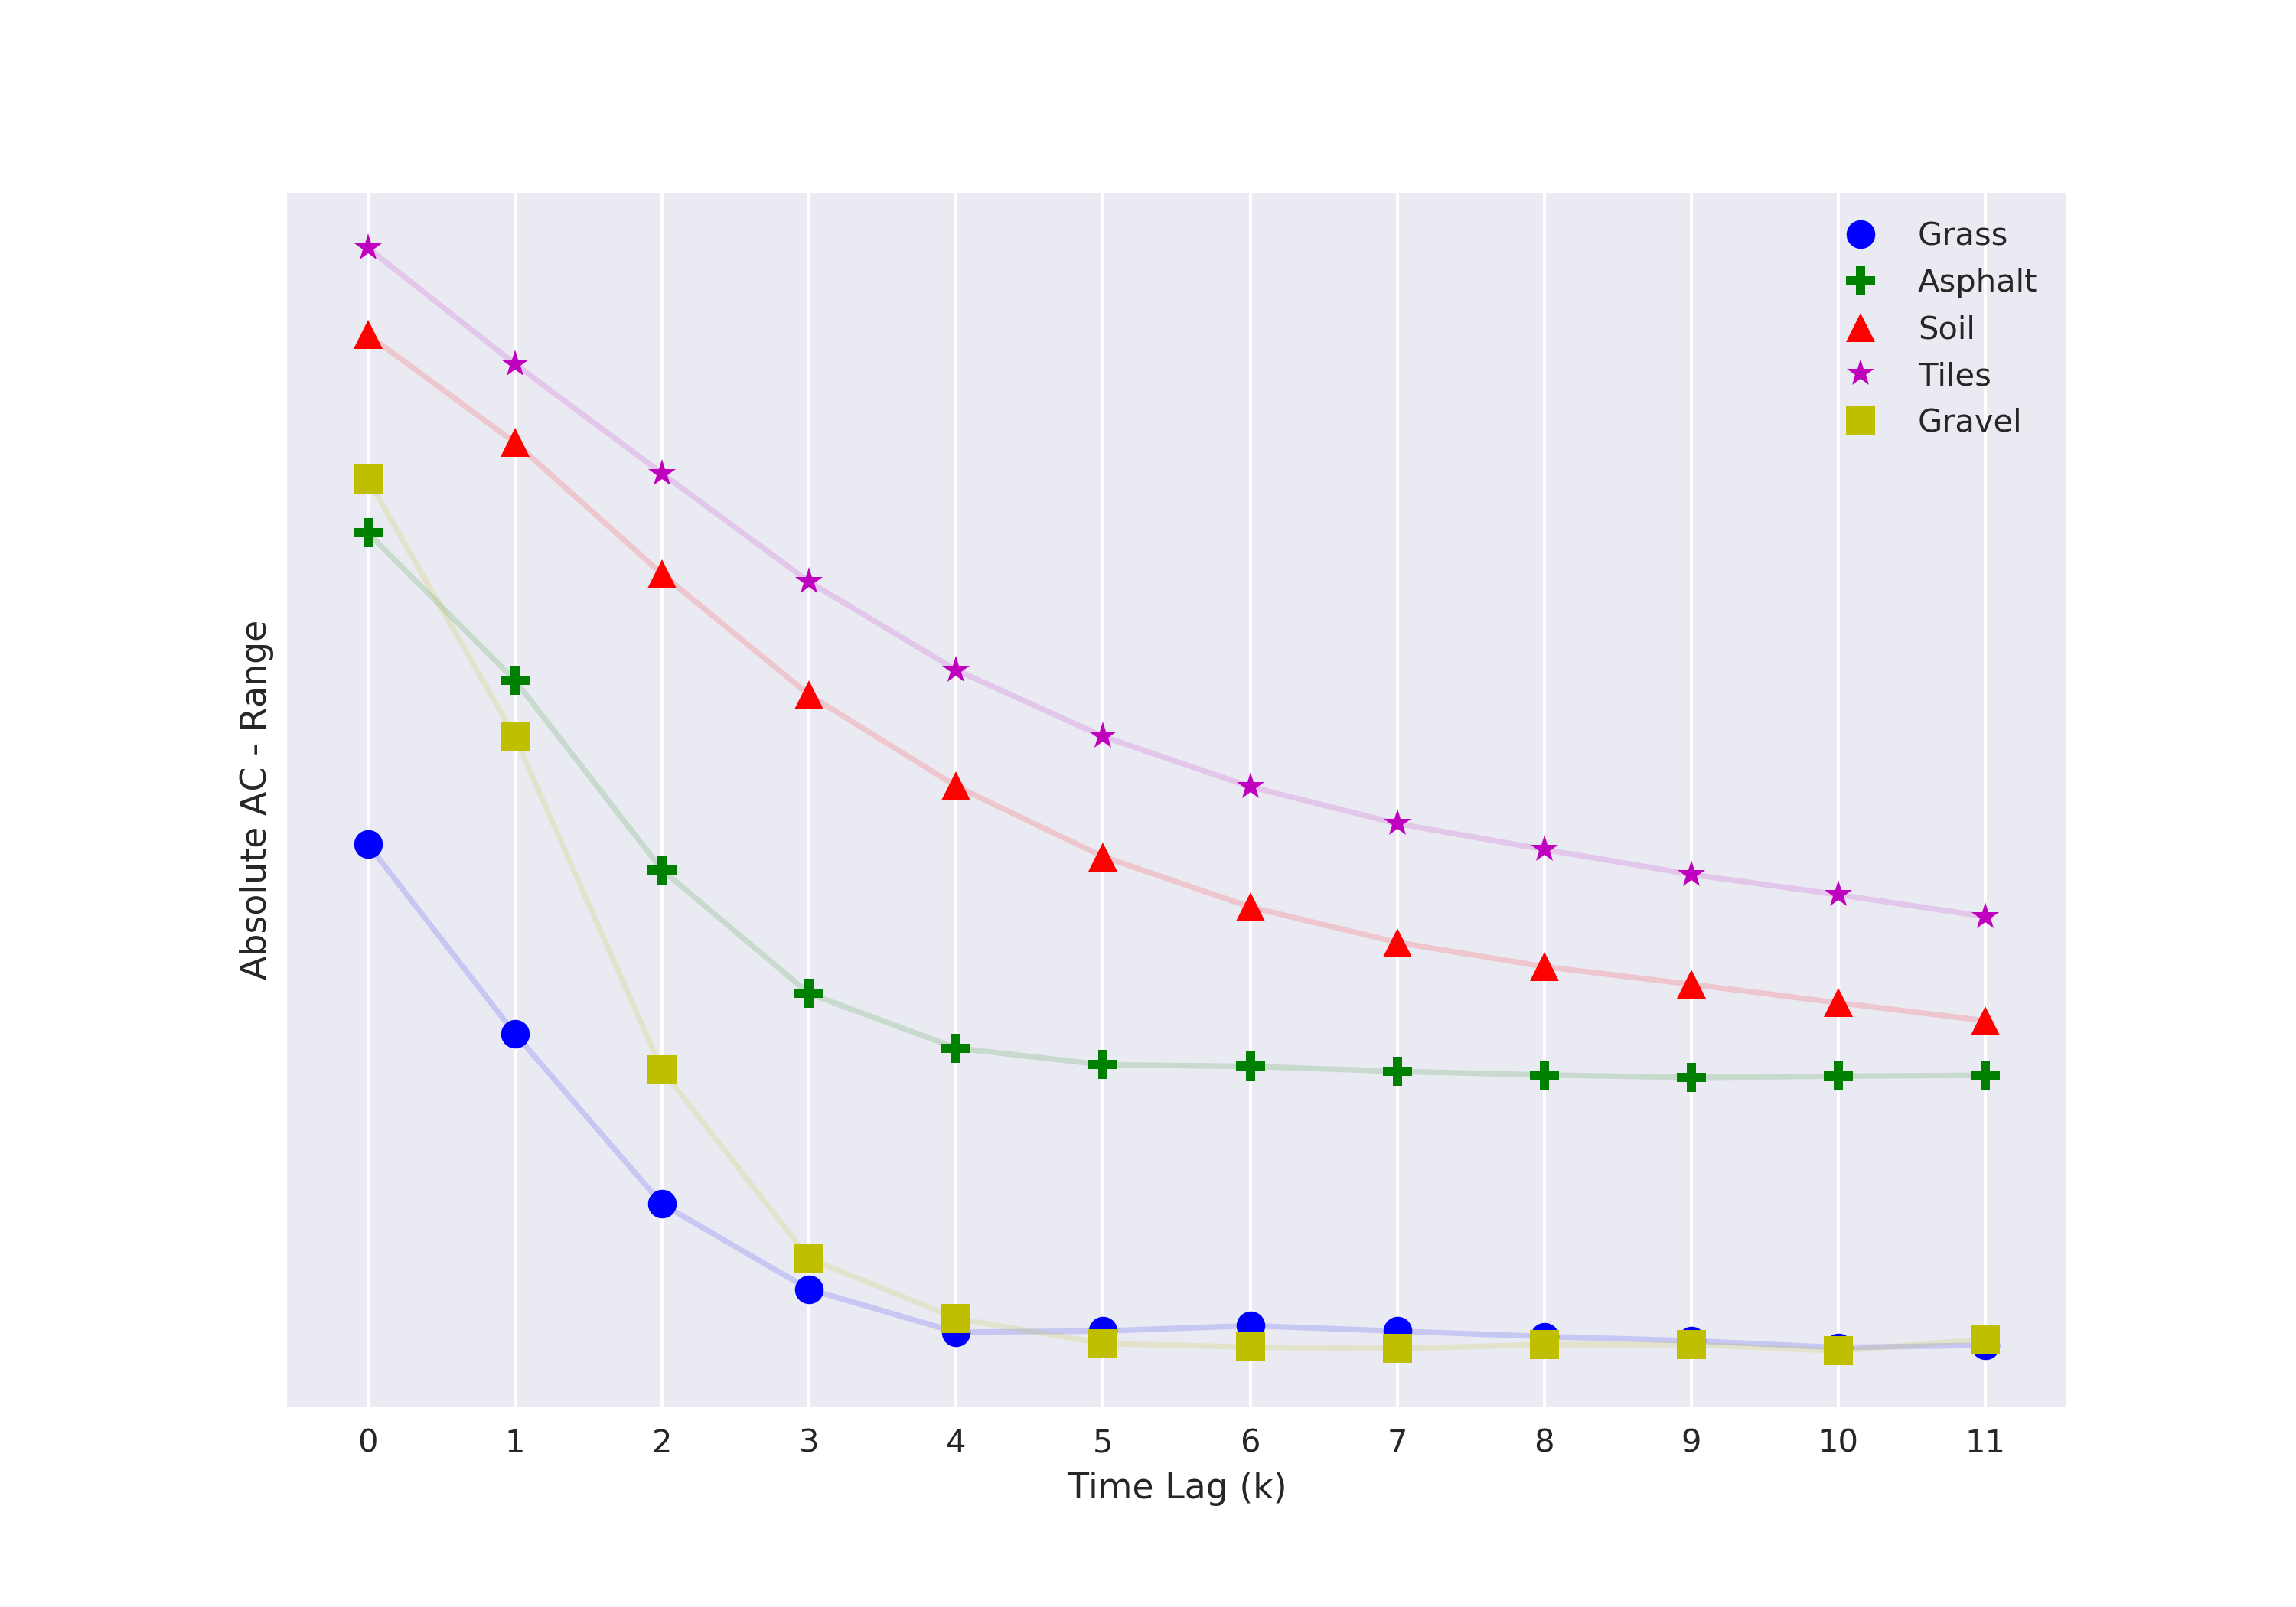
\includegraphics[scale=0.45]{figs_temp/features/autocorr_range.png}
	\caption{The graphs show the autocorrelations computed from time-varying IQ-signals at an appropriate range. The tiled surface, which is the most even, corresponds to the graph with the highest autocorrelation. In contrast, the arguably most uneven surface - grass - is represented by the graph with the lowest autocorrelation.}
	\label{fig:autocorr_range}
\end{figure}


\subsubsection{Autocovariance - energy}

While the sweep normalization process rendered absolute mesurements of signal energy useless, we are still able to investigate its time-dependant structure through the autocovariane function. First we estimate the energy in each sweep $v(t)$ and the average energy $v_a(t)$ in $T$ number of sweeps, and then calculate the real-valued autocovariance sequence $h(m,k)$. 

\begin{equation}
	v(t) = \frac{1}{N}\sum_{n=0}^{K-1}x(n,t)x^*(n,t)
\end{equation}

\begin{equation} 
	v_a(m) = \frac{1}{T}\sum_{t=0}^{T-1}v(t_m+t)
\end{equation}

\begin{equation}
	h(m,k) = \frac{1}{T}\sum_{t=0}^{T-1-k}\big(v(t_m+t) - v_a(m)\big)^*\big(v(t_m+t+k) - v_a(m)\big)
\end{equation}

As $h(m,k)$ only consist of real values, the energy autocovariance feature vector $\mathbf{f}_{h,m}$ is formed as

\begin{equation}
	\mathbf{f}_{h,m} = 
	\begin{bmatrix}
		h(m,0) & h(m,1) & ... & h(m,K-1),
	\end{bmatrix}
\end{equation}
where $K$ is the number of covariance steps included in each sample. 

%We can also calculate the autocovariance function of estimated sweep energy. Although the sweeps are normalized in the preprocessing, we can investigate how the sweeps change over time. 

%The average energy in a sweep tells us how much energy is reflected back to the radar. Hence it can be regarded as a measure of how good of a reflector the underlying surface is. The energy depends on the shape of the surface, as well as its dielectric constant. Compared to other materials, grass has a very different surface shape, which potentially gives it a very different reflexivity. However, its dielectric constant could also vary a lot depending on whether it is wet or dry, making it hard to guess its reflective properties.

%By computing the average energy of single sweeps from different surfaces we see in figure \ref{fig:sweep_energy} that grass reflects much less energy. This indicates that the average sweep energy is a good feature for binary grass/not grass classification. However, in order to get a more robust measure of the average energy we do not only compute the average over selected range bins of a single sweep, but we average over a few consecutive sweeps as well. Mathematically, the feature we end up using becomes
%\begin{equation}
%	P(t_m) = \frac{1}{NT}\sum_{t=0}^{T-1}\sum_{n=0}^{K-1}x(n, t_m + t)x^*(n, t_m + t),
%\end{equation}
%where (describe variables)

%Despite the fact that the average energy appears to be a highly relevant feature, it is also much gain dependent, and conflicts with what is stated in section *reference to sweep norm.*. Therefore, if different sensors are to be used for training and future classifications, this feature will not be of any use.


\begin{table}
\label{tab:feat}
\begin{center}
\rowcolors{2}{gray!25}{white}
  \begin{tabular}{|c|cccccc|}
\hline
    \rowcolor{gray!150}
		  & \color{white}\textbf{Abs} & \color{white}\textbf{AC Energy} & \color{white}\textbf{AC Range} & \color{white}\textbf{FFT} & \color{white}\textbf{Features} & \color{white}\textbf{Accuracy} \\
	  Config 1 & X &   &   &   & 28  & 94.49 \\
	  Config 2 & X & X & X & & 175 & 98.49 \\
	  Config 3 & & & & X & 700 & 98.38 \\
\hline
  \end{tabular}
\end{center}
\caption{Feature configurations}
\end{table}


\subsection{Tested feature combinations}

In above section, four different features were described - the average signal shape, the autocovariance in range, the autocovariance in energy and the fourier transform. These methods each generate a number of features. However, we are not limited to feed our model with features taken from a single one of the feature extraction methods. In table \ref{tab:feat} three possible configurations of features are chosen. Each of these combinations were fed through the same classifier to evaluate which was the most efficient. The first one, which simply involves the averaged signal shape, requires much fewer features than the other two combinations. But looking at its performance, these features are not enough to reach the accuracy attained in the other two cases. By appending the autocovariances for ranges as well as for sweep energy, the accuracy increases by 4 percentage points. 

We can also choose to look at the Fourier transform, as in configuration 3. In this case, we omit both the averaged signal shape as well as the autocovariances. The reason is that the Fourier transform is based on the original IQ-data, and by applying the inverse Fourier transform we can go back to the original data. Hence no information is lost, and the information about signal shape and autocovariances remains and can be found by, for instance a neural network, if necessary\footnote{With a neural network complex enough, raw IQ-data could be feeded to the network and it would eventually find any relevant features on its own. But by manually preprocessing the data the convergence rate and complexity of the neural network can be reduced.}. With these features we reach a slightly lower accuracy than configuration 2, but more importantly we would need 700 features compared to 175, making configuration 2 much more favorable as it demands less computational costs. Hence configuration 2 is deemed the most efficient.


\section{Feature Principal Component Analysis}

Through the point and feature selection methods described in previous sections we obtain high dimensional feature vectors. Getting an intuitive feel for such data extracted in these processes is difficult as direct plotting is limited to three dimensions. 

Principal Component Analysis (PCA) is  a classical technique in statistical data analysis which takes a large set variables from a multivariate dataset and finds a smaller set of variables with less redundancy. Critically, PCA finds a rotated orthogonal coordinate system such that the elements of the set become uncorrelated. Projecting elements on the principal axes corresponding to the directions of maximal variance a good approximation of the original data in lower dimension is obtained \citep{hyvasrinen_karhunen_oja_2004}.

After having chosen to proceed with feature configuration 2 in table \ref{tab:feat}, the 175 dimensions can be reduced to 2 dimensions using PCA. This helps to visualize the separability of the different materials as seen in figure \ref{fig:pca}.

\begin{figure}[h]
	\centering
	\includegraphics[scale=0.55]{figs_temp/pca_analysis.png}
	\caption{By performing a principal component analysis on the feature vectors we may reduce them from a 175-dimensional space into 2 dimensions, maintaining maximal variance. This allows us to visualize, and get an idea of how separable the materials are.}
	\label{fig:pca}
\end{figure}

